\documentclass[a4paper,12pt]{article}

\usepackage[margin=2cm]{geometry}
\usepackage{mathrsfs}
\usepackage[svgnames]{xcolor}
\usepackage{tikz}
\usepackage{tkz-base}


% Début du document
%%%%%%%%%%%%%%%%%%%
\begin{document}

\section{Quelques exemples}

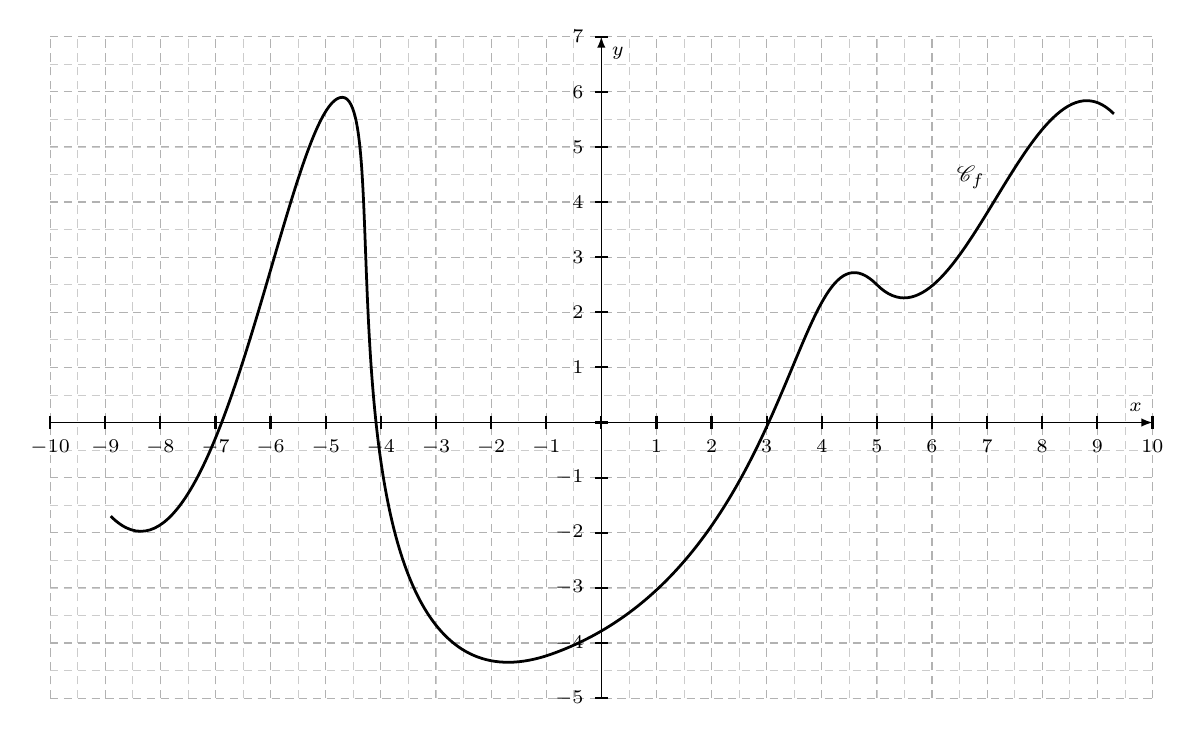
\begin{tikzpicture}[scale=0.7]
	%
	% Limites du repère modifiables
	\def\bezierXmin{-10}
	\def\bezierXmax{10}
	\def\bezierYmin{-5}
	\def\bezierYmax{7}
	%
	% Grille
	\draw[step=0.5,densely dashed,line width=0.25pt,draw=black!20] (\bezierXmin,\bezierYmin) grid (\bezierXmax,\bezierYmax);
	\draw[step=1,densely dashed,line width=0.4pt,draw=black!30] (\bezierXmin,\bezierYmin) grid (\bezierXmax,\bezierYmax);
	%
	% Création des axes avec tkz-base
	\tkzInit[xmin=\bezierXmin,xmax=\bezierXmax,ymin=\bezierYmin,ymax=\bezierYmax]
	\tkzSetUpAxis[ticka=3.5pt,tickb=3.5pt]	%Taille graduations
	\tkzLabelX[font=\scriptsize,orig=false,fill=none] % Graduations X 
	\tkzLabelY[font=\scriptsize,orig=false,fill=none] % Graduations Y
	\tkzDrawX[right space=0pt,above left=4pt,font=\scriptsize] %Axe X
	\tkzDrawY[up space=0pt,below right=4pt,font=\scriptsize] %Axe Y
	\clip (\bezierXmin,\bezierYmin) rectangle (\bezierXmax,\bezierYmax);
	%
	% Courbe
	%
	\draw[line width=1pt] (-8.9,-1.7) .. controls (-6.9,-3.7) and (-5.7,5.9) .. (-4.7,5.9) .. controls (-3.7,5.9) and (-5.4,-5.8) .. (-0.9,-4.2) .. controls (3.6,-2.6) and (3.5,4) .. (5,2.5) .. controls (6.5,1) and (7.8,7.1) .. (9.3,5.6) node[font=\footnotesize,pos=0.5,above left] {$\mathscr C_f$};
\end{tikzpicture}

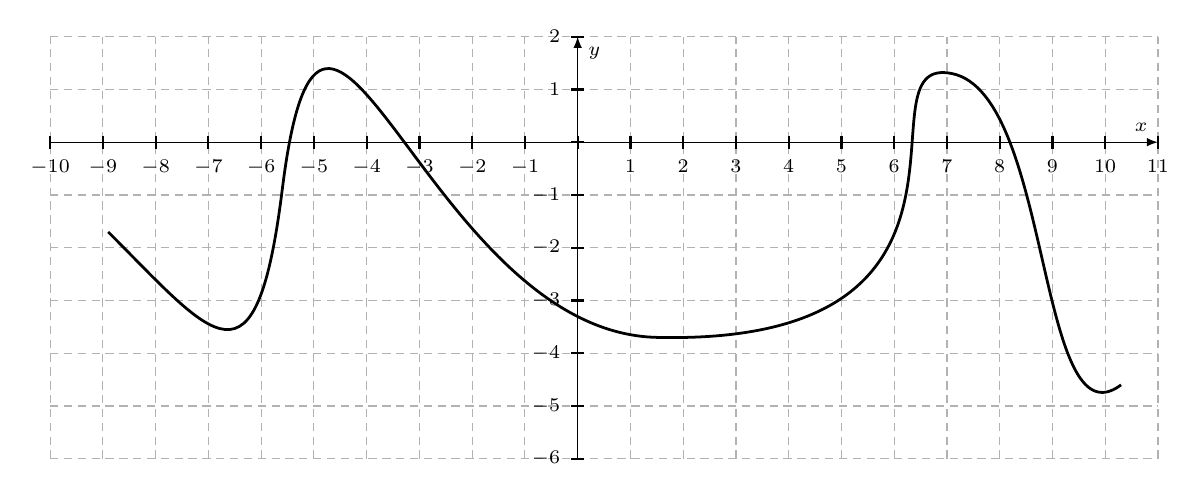
\begin{tikzpicture}[scale=0.67]
	%
	% Limites du repère modifiables
	\def\bezierXmin{-10}
	\def\bezierXmax{11}
	\def\bezierYmin{-6}
	\def\bezierYmax{2}
	%
	% Grille
	\draw[step=1,densely dashed,line width=0.4pt,draw=black!30] (\bezierXmin,\bezierYmin) grid (\bezierXmax,\bezierYmax);
	%
	% Création des axes avec tkz-base
	\tkzInit[xmin=\bezierXmin,xmax=\bezierXmax,ymin=\bezierYmin,ymax=\bezierYmax]
	\tkzSetUpAxis[ticka=3.5pt,tickb=3.5pt]	%Taille graduations
	\tkzLabelX[font=\scriptsize,orig=false,fill=none] % Graduations X 
	\tkzLabelY[font=\scriptsize,orig=false,fill=none] % Graduations Y
	\tkzDrawX[right space=0pt,above left=4pt,font=\scriptsize] %Axe X
	\tkzDrawY[up space=0pt,below right=4pt,font=\scriptsize] %Axe Y
	\clip (\bezierXmin,\bezierYmin) rectangle (\bezierXmax,\bezierYmax);
	%
	% Courbe
	%
	\draw[line width=1pt] (-8.9,-1.7) .. controls (-6.9,-3.7) and (-6.1,-4.9) .. (-5.6,-0.9) .. controls (-4.8,5.54) and (-2.9,-3.6) .. (1.5,-3.7) .. controls (8.46,-3.86) and (5.2,1.7) .. (7.1,1.3) .. controls (9,0.9) and (8.7,-5.8) .. (10.3,-4.6);
\end{tikzpicture}

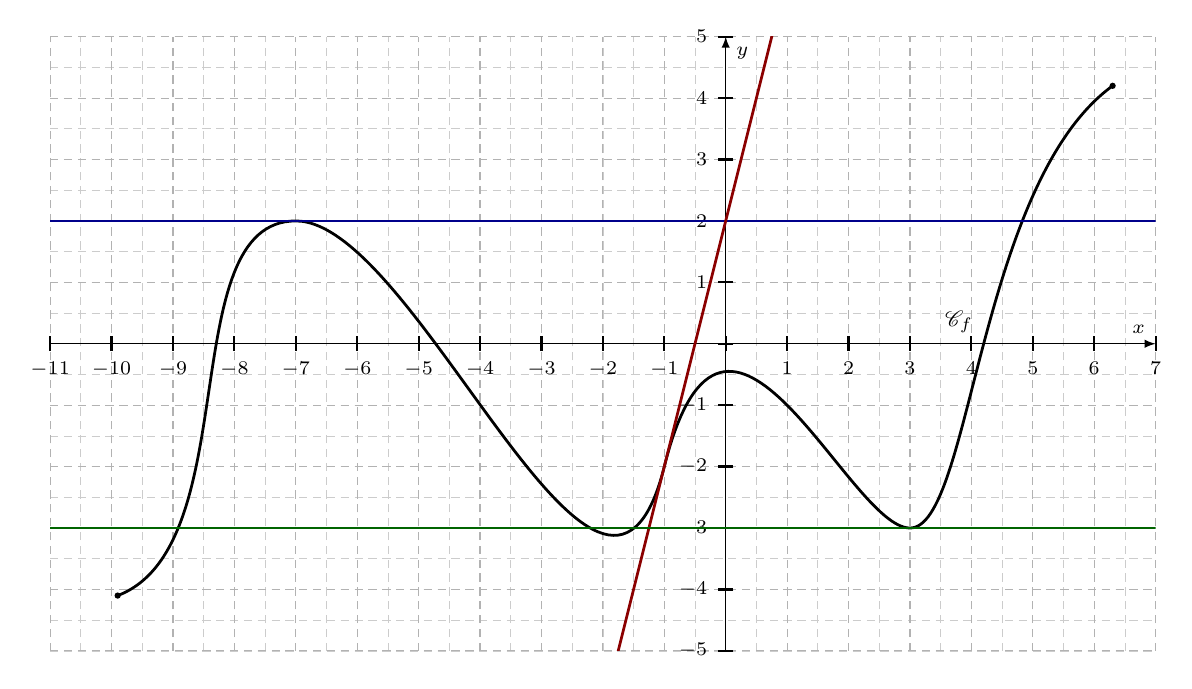
\begin{tikzpicture}[scale=0.78]
	%
	% Limites du repère modifiables
	\def\bezierXmin{-11}
	\def\bezierXmax{7}
	\def\bezierYmin{-5}
	\def\bezierYmax{5}
	%
	% Grille
	\draw[step=0.5,densely dashed,line width=0.25pt,draw=black!20] (\bezierXmin,\bezierYmin) grid (\bezierXmax,\bezierYmax);
	\draw[step=1,densely dashed,line width=0.4pt,draw=black!30] (\bezierXmin,\bezierYmin) grid (\bezierXmax,\bezierYmax);
	%
	% Création des axes avec tkz-base
	\tkzInit[xmin=\bezierXmin,xmax=\bezierXmax,ymin=\bezierYmin,ymax=\bezierYmax]
	\tkzSetUpAxis[ticka=3.5pt,tickb=3.5pt]	%Taille graduations
	\tkzLabelX[font=\scriptsize,orig=false,fill=none] % Graduations X 
	\tkzLabelY[font=\scriptsize,orig=false,fill=none] % Graduations Y
	\tkzDrawX[right space=0pt,above left=4pt,font=\scriptsize] %Axe X
	\tkzDrawY[up space=0pt,below right=4pt,font=\scriptsize] %Axe Y
	\clip (\bezierXmin,\bezierYmin) rectangle (\bezierXmax,\bezierYmax);
	%
	% Courbe
	%
	\draw[line width=1pt] (-9.9,-4.1) .. controls (-7.8,-3.3) and (-9,2) .. (-7,2) node[pos=0,circle,fill,inner sep=0.8pt] {} .. controls (-5,2) and (-2,-6) .. (-1,-2) .. controls (0,2) and (2,-3) .. (3,-3) .. controls (4,-3) and (4.1,2.6) .. (6.3,4.2) node[font=\footnotesize,pos=0.5,above left] {$\mathscr C_f$} node[pos=1,circle,fill,inner sep=0.8pt] {};
	%
	% Tangentes
	\draw[domain=\bezierXmin:\bezierXmax,line width=1pt,DarkBlue] plot (\x,{0/2*\x+2});
	\draw[domain=\bezierXmin:\bezierXmax,line width=1pt,DarkRed] plot (\x,{4/1*\x+2});
	\draw[domain=\bezierXmin:\bezierXmax,line width=1pt,DarkGreen] plot (\x,{0/1*\x-3});
\end{tikzpicture}

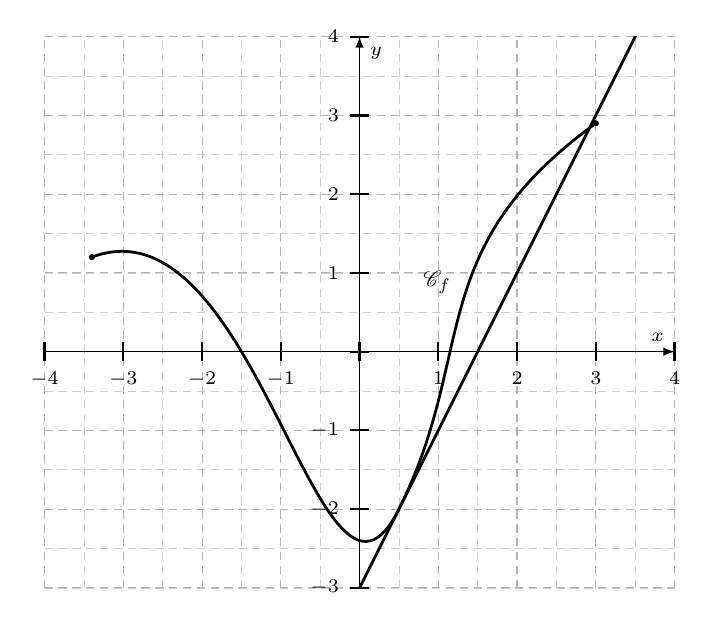
\begin{tikzpicture}
	%
	% Limites du repère modifiables
	\def\bezierXmin{-4}
	\def\bezierXmax{4}
	\def\bezierYmin{-3}
	\def\bezierYmax{4}
	%
	% Grille
	\draw[step=0.5,densely dashed,line width=0.25pt,draw=black!20] (\bezierXmin,\bezierYmin) grid (\bezierXmax,\bezierYmax);
	\draw[step=1,densely dashed,line width=0.4pt,draw=black!30] (\bezierXmin,\bezierYmin) grid (\bezierXmax,\bezierYmax);
	%
	% Création des axes avec tkz-base
	\tkzInit[xmin=\bezierXmin,xmax=\bezierXmax,ymin=\bezierYmin,ymax=\bezierYmax]
	\tkzSetUpAxis[ticka=3.5pt,tickb=3.5pt]	%Taille graduations
	\tkzLabelX[font=\scriptsize,orig=false,fill=none] % Graduations X 
	\tkzLabelY[font=\scriptsize,orig=false,fill=none] % Graduations Y
	\tkzDrawX[right space=0pt,above left=4pt,font=\scriptsize] %Axe X
	\tkzDrawY[up space=0pt,below right=4pt,font=\scriptsize] %Axe Y
	\clip (\bezierXmin,\bezierYmin) rectangle (\bezierXmax,\bezierYmax);
	%
	% Courbe
	%
	\draw[line width=1pt] (-3.4,1.2) .. controls (-1.3,2) and (-0.5,-4) .. (0.5,-2) node[pos=0,circle,fill,inner sep=0.8pt] {} .. controls (1.5,0) and (0.8,1.3) .. (3,2.9) node[font=\footnotesize,pos=0.5,above left] {$\mathscr C_f$} node[pos=1,circle,fill,inner sep=0.8pt] {};
	%
	% Tangentes
	\draw[domain=\bezierXmin:\bezierXmax,line width=1pt] plot (\x,{2/1*\x-3});
\end{tikzpicture}

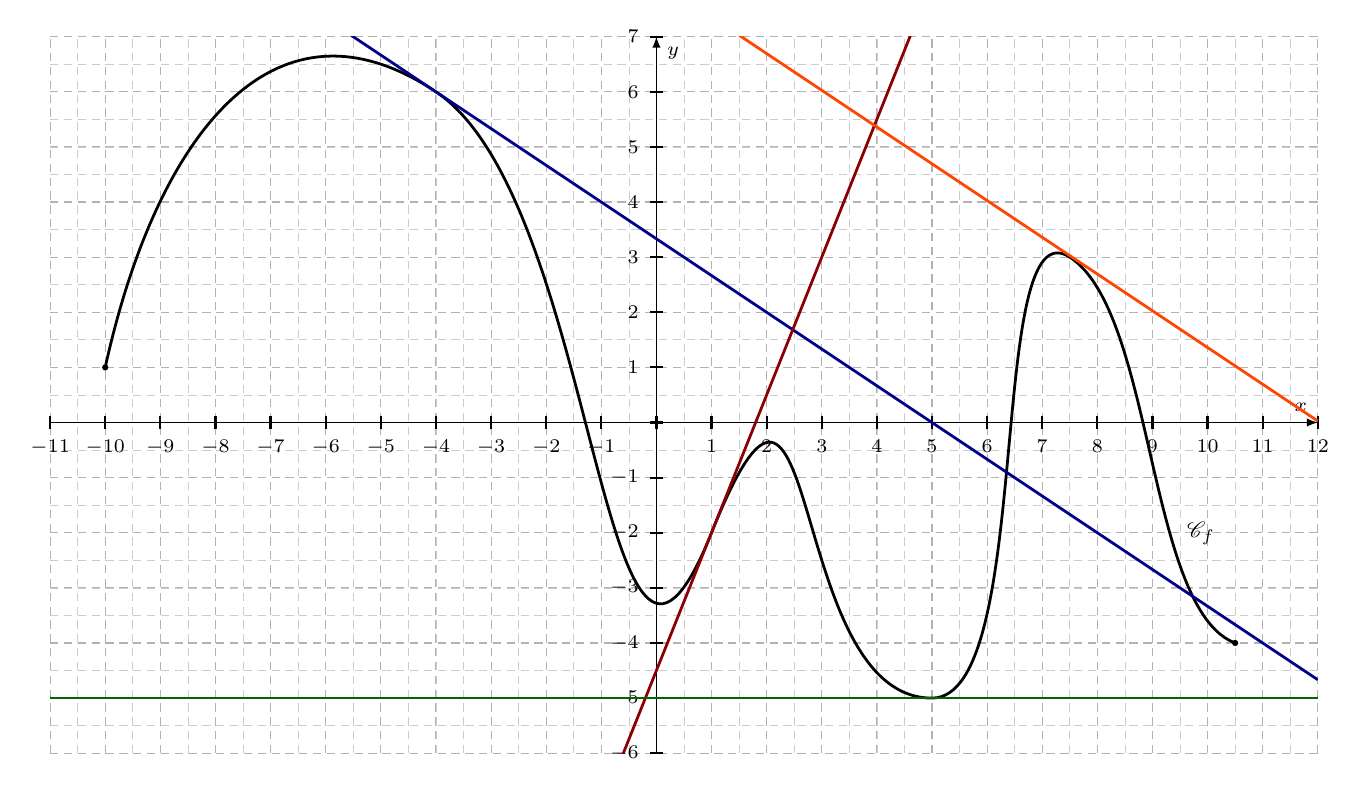
\begin{tikzpicture}[scale=0.7]
	%
	% Limites du repère modifiables
	\def\bezierXmin{-11}
	\def\bezierXmax{12}
	\def\bezierYmin{-6}
	\def\bezierYmax{7}
	%
	% Grille
	\draw[step=0.5,densely dashed,line width=0.25pt,draw=black!20] (\bezierXmin,\bezierYmin) grid (\bezierXmax,\bezierYmax);
	\draw[step=1,densely dashed,line width=0.4pt,draw=black!30] (\bezierXmin,\bezierYmin) grid (\bezierXmax,\bezierYmax);
	%
	% Création des axes avec tkz-base
	\tkzInit[xmin=\bezierXmin,xmax=\bezierXmax,ymin=\bezierYmin,ymax=\bezierYmax]
	\tkzSetUpAxis[ticka=3.5pt,tickb=3.5pt]	%Taille graduations
	\tkzLabelX[font=\scriptsize,orig=false,fill=none] % Graduations X 
	\tkzLabelY[font=\scriptsize,orig=false,fill=none] % Graduations Y
	\tkzDrawX[right space=0pt,above left=4pt,font=\scriptsize] %Axe X
	\tkzDrawY[up space=0pt,below right=4pt,font=\scriptsize] %Axe Y
	\clip (\bezierXmin,\bezierYmin) rectangle (\bezierXmax,\bezierYmax);
	%
	% Courbe
	%
	\draw[line width=1pt] (-10,1) .. controls (-9.1,5.1) and (-7,8) .. (-4,6) node[pos=0,circle,fill,inner sep=0.8pt] {} .. controls (-1,4) and (-1,-7) .. (1,-2) .. controls (3,3) and (2.3,-5) .. (5,-5) .. controls (6.88,-5) and (5.96,4) .. (7.5,3) .. controls (9.04,2) and (8.9,-3.4) .. (10.5,-4) node[font=\footnotesize,pos=0.7,above right] {$\mathscr C_f$} node[pos=1,circle,fill,inner sep=0.8pt] {};
	%
	% Tangentes
	\draw[domain=\bezierXmin:\bezierXmax,line width=1pt,DarkBlue] plot (\x,{-2/3*\x+3.333});
	\draw[domain=\bezierXmin:\bezierXmax,line width=1pt,DarkRed] plot (\x,{5/2*\x-4.5});
	\draw[domain=\bezierXmin:\bezierXmax,line width=1pt,DarkGreen] plot (\x,{0/1.9*\x-5});
	\draw[domain=\bezierXmin:\bezierXmax,line width=1pt,OrangeRed] plot (\x,{-1/1.5*\x+8.027});
\end{tikzpicture}

\section{Un exemple de courbe non régulière}

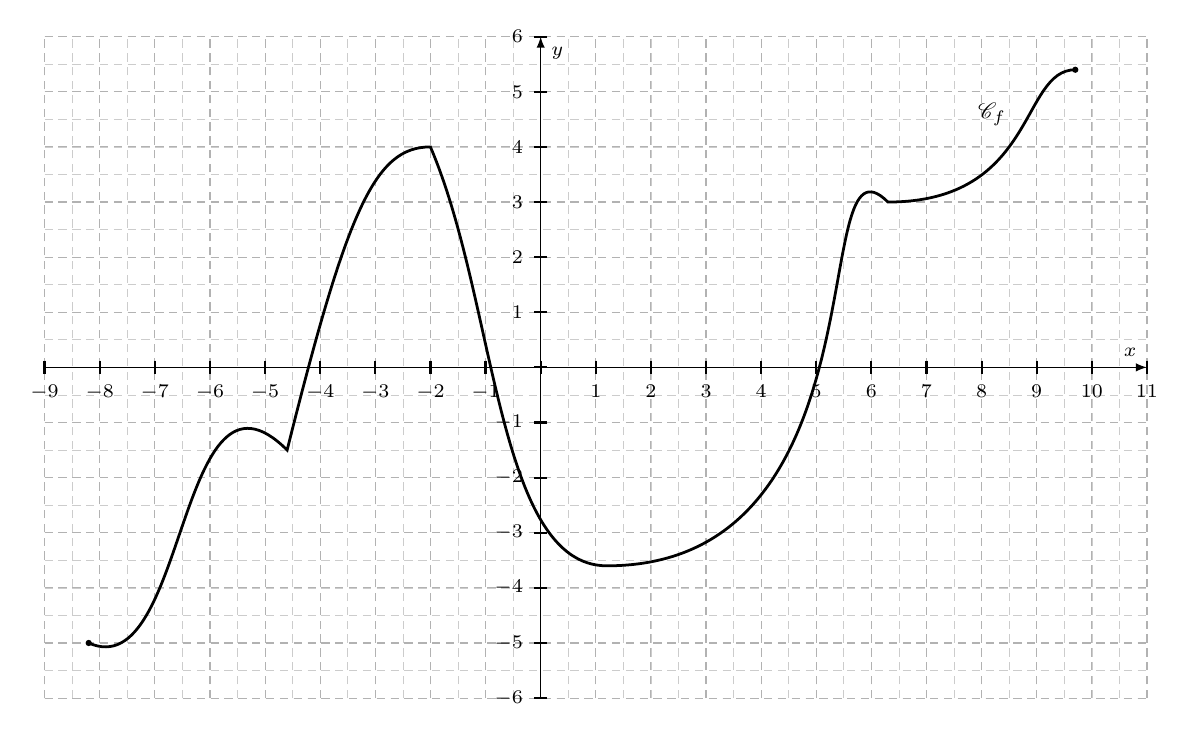
\begin{tikzpicture}[scale=0.7]
	%
	% Limites du repère modifiables
	\def\bezierXmin{-9}
	\def\bezierXmax{11}
	\def\bezierYmin{-6}
	\def\bezierYmax{6}
	%
	% Grille
	\draw[step=0.5,densely dashed,line width=0.25pt,draw=black!20] (\bezierXmin,\bezierYmin) grid (\bezierXmax,\bezierYmax);
	\draw[step=1,densely dashed,line width=0.4pt,draw=black!30] (\bezierXmin,\bezierYmin) grid (\bezierXmax,\bezierYmax);
	%
	% Création des axes avec tkz-base
	\tkzInit[xmin=\bezierXmin,xmax=\bezierXmax,ymin=\bezierYmin,ymax=\bezierYmax]
	\tkzSetUpAxis[ticka=3.5pt,tickb=3.5pt]	%Taille graduations
	\tkzLabelX[font=\scriptsize,orig=false,fill=none] % Graduations X 
	\tkzLabelY[font=\scriptsize,orig=false,fill=none] % Graduations Y
	\tkzDrawX[right space=0pt,above left=4pt,font=\scriptsize] %Axe X
	\tkzDrawY[up space=0pt,below right=4pt,font=\scriptsize] %Axe Y
	\clip (\bezierXmin,\bezierYmin) rectangle (\bezierXmax,\bezierYmax);
	%
	% Courbe
	%
	\draw[line width=1pt] (-8.2,-5) .. controls (-6.4,-5.8) and (-6.6,0.5) .. (-4.6,-1.5) node[pos=0,circle,fill,inner sep=0.8pt] {} .. controls (-3.5,2.9) and (-3,4) .. (-2,4) .. controls (-0.8,1.2) and (-0.8,-3.6) .. (1.2,-3.6) .. controls (6.36,-3.6) and (4.8,4.5) .. (6.3,3) .. controls (9,3) and (8.7,5.4) .. (9.7,5.4) node[font=\footnotesize,pos=0.5,above left] {$\mathscr C_f$} node[pos=1,circle,fill,inner sep=0.8pt] {};
\end{tikzpicture}

\section{Une courbe quelconque}

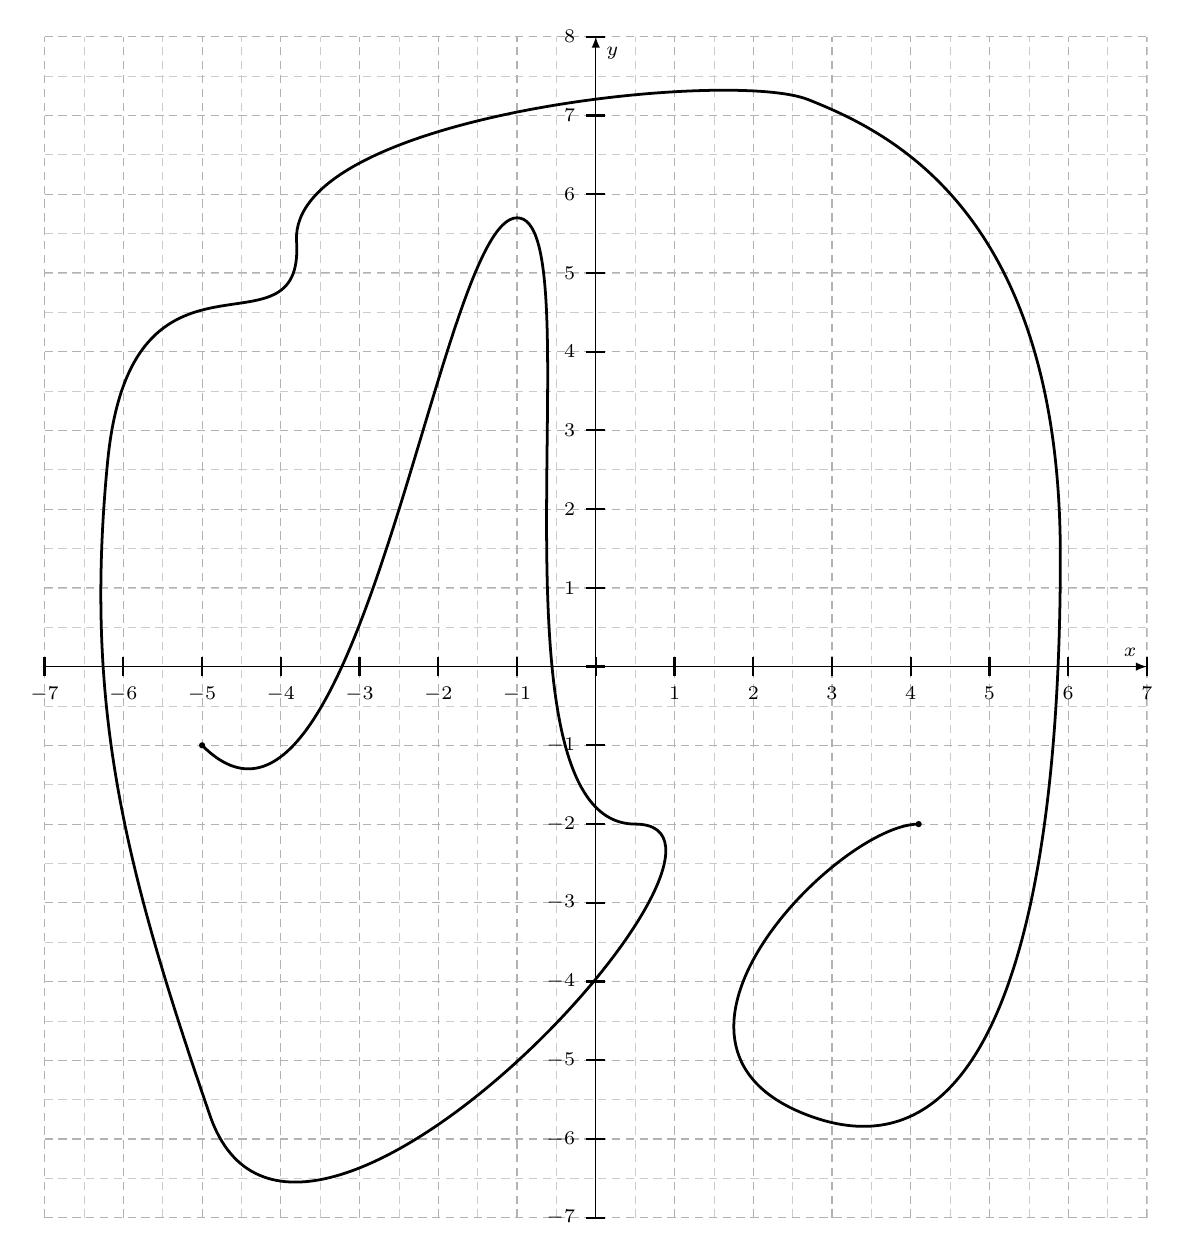
\begin{tikzpicture}
	%
	% Limites du repère modifiables
	\def\bezierXmin{-7}
	\def\bezierXmax{7}
	\def\bezierYmin{-7}
	\def\bezierYmax{8}
	%
	% Grille
	\draw[step=0.5,densely dashed,line width=0.25pt,draw=black!20] (\bezierXmin,\bezierYmin) grid (\bezierXmax,\bezierYmax);
	\draw[step=1,densely dashed,line width=0.4pt,draw=black!30] (\bezierXmin,\bezierYmin) grid (\bezierXmax,\bezierYmax);
	%
	% Création des axes avec tkz-base
	\tkzInit[xmin=\bezierXmin,xmax=\bezierXmax,ymin=\bezierYmin,ymax=\bezierYmax]
	\tkzSetUpAxis[ticka=3.5pt,tickb=3.5pt]	%Taille graduations
	\tkzLabelX[font=\scriptsize,orig=false,fill=none] % Graduations X 
	\tkzLabelY[font=\scriptsize,orig=false,fill=none] % Graduations Y
	\tkzDrawX[right space=0pt,above left=4pt,font=\scriptsize] %Axe X
	\tkzDrawY[up space=0pt,below right=4pt,font=\scriptsize] %Axe Y
	\clip (\bezierXmin,\bezierYmin) rectangle (\bezierXmax,\bezierYmax);
	%
	% Courbe
	%
	\draw[line width=1pt] (-5,-1) .. controls (-3,-3) and (-2,5.7) .. (-1,5.7) node[pos=0,circle,fill,inner sep=0.8pt] {} .. controls (0,5.7) and (-1.5,-2) .. (0.5,-2) .. controls (2.5,-2) and (-3.8,-8.9) .. (-4.9,-5.7) .. controls (-6,-2.5) and (-6.5,-0.5) .. (-6.2,2.6) .. controls (-5.9,5.7) and (-3.7,3.8) .. (-3.8,5.4) .. controls (-3.9,7) and (1.7,7.6) .. (2.7,7.2) .. controls (3.7,6.8) and (5.9,5.8) .. (5.9,1.4) .. controls (5.9,-3) and (5.1,-6.6) .. (2.7,-5.7) .. controls (0.3,-4.8) and (3.1,-2) .. (4.1,-2) node[pos=1,circle,fill,inner sep=0.8pt] {};
\end{tikzpicture}

\section{Deux courbes}

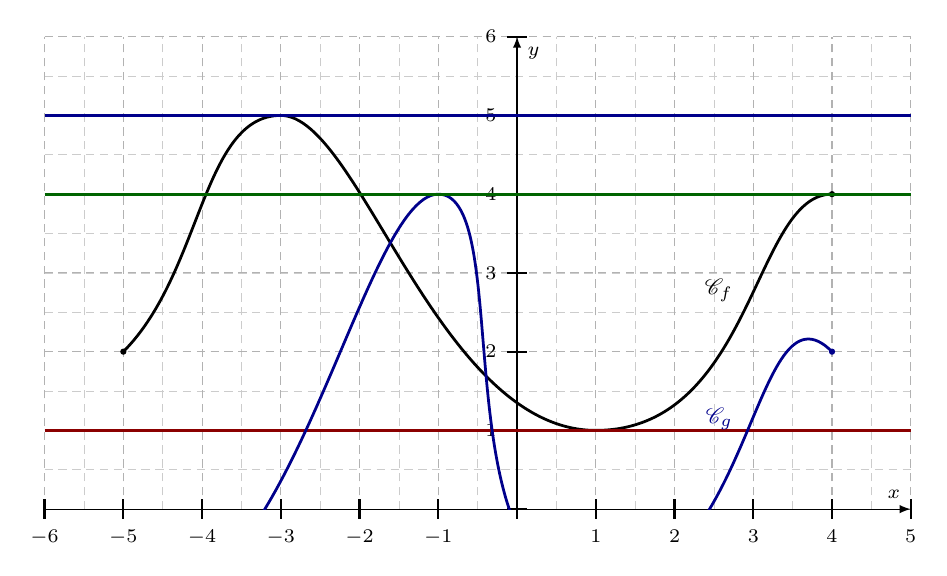
\begin{tikzpicture}
	%
	% Limites du repère modifiables
	\def\bezierXmin{-6}
	\def\bezierXmax{5}
	\def\bezierYmin{0}
	\def\bezierYmax{6}
	%
	% Grille
	\draw[step=0.5,densely dashed,line width=0.25pt,draw=black!20] (\bezierXmin,\bezierYmin) grid (\bezierXmax,\bezierYmax);
	\draw[step=1,densely dashed,line width=0.4pt,draw=black!30] (\bezierXmin,\bezierYmin) grid (\bezierXmax,\bezierYmax);
	%
	% Création des axes avec tkz-base
	\tkzInit[xmin=\bezierXmin,xmax=\bezierXmax,ymin=\bezierYmin,ymax=\bezierYmax]
	\tkzSetUpAxis[ticka=3.5pt,tickb=3.5pt]	%Taille graduations
	\tkzLabelX[font=\scriptsize,orig=false,fill=none] % Graduations X 
	\tkzLabelY[font=\scriptsize,orig=false,fill=none] % Graduations Y
	\tkzDrawX[right space=0pt,above left=4pt,font=\scriptsize] %Axe X
	\tkzDrawY[up space=0pt,below right=4pt,font=\scriptsize] %Axe Y
	\clip (\bezierXmin,\bezierYmin) rectangle (\bezierXmax,\bezierYmax);
	%
	% Courbes
	%
	\draw[line width=1pt,black] (-5,2) .. controls (-4,3) and (-4,5) .. (-3,5) node[pos=0,circle,fill,inner sep=0.8pt] {} .. controls (-2,5) and (-1,1) .. (1,1) .. controls (3,1) and (3,4) .. (4,4) node[font=\footnotesize,pos=0.5,above left] {$\mathscr C_f$} node[pos=1,circle,fill,inner sep=0.8pt] {};
	% Tangentes
	\draw[domain=\bezierXmin:\bezierXmax,line width=1pt,DarkBlue] plot (\x,{0/1*\x+5});
	\draw[domain=\bezierXmin:\bezierXmax,line width=1pt,DarkRed] plot (\x,{0/2*\x+1});
	%
	% Courbe 2
	\draw[line width=1pt,DarkBlue] (-5,-1) .. controls (-3,-2) and (-2,4) .. (-1,4) node[pos=0,circle,fill,inner sep=0.8pt] {} .. controls (0,4) and (-1,-1) .. (1,-1) .. controls (3,-1) and (3,3) .. (4,2) node[font=\footnotesize,pos=0.5,above left] {$\mathscr C_g$} node[pos=1,circle,fill,inner sep=0.8pt] {};
	% Tangentes
	\draw[domain=\bezierXmin:\bezierXmax,line width=1pt,DarkGreen] plot (\x,{0/1*\x+4});
	\draw[domain=\bezierXmin:\bezierXmax,line width=1pt,OrangeRed] plot (\x,{0/2*\x-1});
\end{tikzpicture}

\end{document}
